\subsubsection{Module MD-03: Quản lý Đặt chỗ \& Đặt món trước}
Module Quản lý Đặt chỗ \& Đặt món trước (MD-03) được thiết kế để cung cấp một giải pháp toàn diện cho nhà hàng trong việc quản lý các yêu cầu đặt bàn từ khách hàng, cả qua kênh trực tuyến lẫn các kênh truyền thống. Module này không chỉ giúp tối ưu hóa việc sử dụng không gian và nguồn lực của nhà hàng mà còn nâng cao trải nghiệm của khách hàng bằng cách cho phép họ chủ động tìm kiếm, lựa chọn thời gian, bàn (tùy chọn), và thậm chí đặt trước các món ăn mong muốn.



\begin{figure}[H]
    \centering
    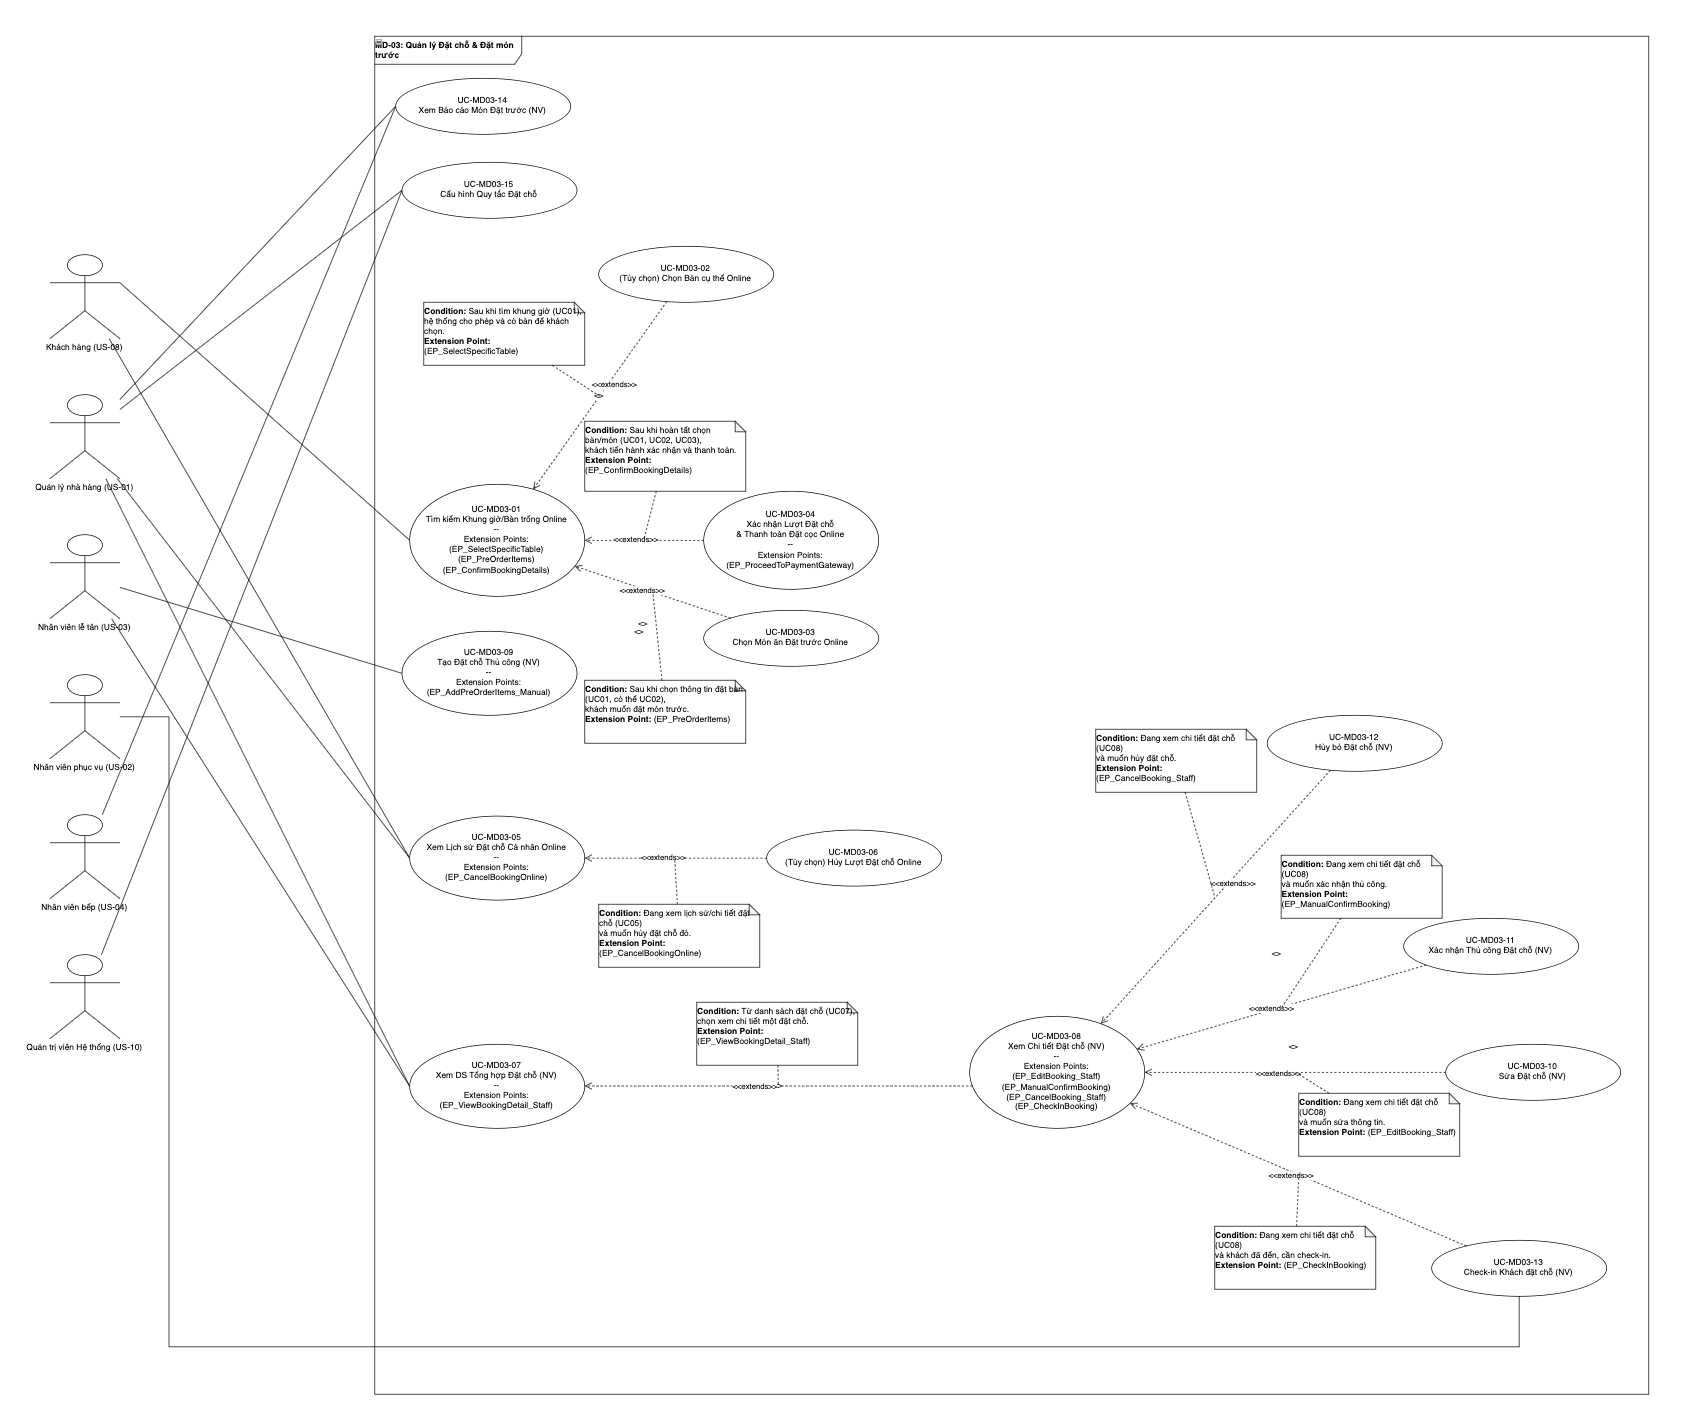
\includegraphics[width=15cm]{Sections/tong_quan/functional_spec/img/uc3.png}
    \vspace{0.5cm}
    \caption{Use case diagram cho Module MD-03}
    \label{fig:my_label}
\end{figure}

\begin{longtable}{|m{2cm}|m{2.5cm}|m{2cm}|m{4.5cm}|m{4cm}|}
\caption{Danh sách Yêu cầu Chức năng cho Module MD-03: Quản lý Đặt chỗ \& Đặt món trước} \label{tab:fr_md03_revised_v3} \\
\hline
\textbf{Mã Module} & \textbf{Mã Yêu cầu CN} & \textbf{Mã Người dùng} & \textbf{Tên Chức năng} & \textbf{Mô tả Ngắn} \\
\hline
\endhead % Header cho các trang tiếp theo
\hline
\endfoot % Footer cho bảng
\hline
\endlastfoot % Footer cho trang cuối cùng

% === Luồng Khách hàng Đặt Online ===
MD-03 & FR-MD03-01 & US-08 & Tìm kiếm Khung giờ/Bàn trống Online & Khách hàng nhập ngày, giờ, số người để tìm kiếm các lựa chọn đặt bàn còn trống. \\
\hline
MD-03 & FR-MD03-02 & US-08 & (Tùy chọn) Chọn Bàn cụ thể từ Sơ đồ tầng Online & Khách hàng xem sơ đồ và chọn bàn trống cụ thể (nếu được phép). \\
\hline
MD-03 & FR-MD03-03 & US-08 & Chọn Món ăn Đặt trước từ Thực đơn Online & Khách hàng duyệt thực đơn và thêm các món muốn đặt trước vào giỏ hàng. \\
\hline
MD-03 & FR-MD03-04 & US-08 & Xác nhận Lượt Đặt chỗ và Thanh toán Đặt cọc Online & Khách hàng xem lại toàn bộ thông tin, nhập thông tin cá nhân và thực hiện thanh toán tiền đặt cọc. \\
\hline
MD-03 & FR-MD03-05 & US-08 & Xem Lịch sử Đặt chỗ Cá nhân Online & Khách hàng đã đăng nhập xem lại các đặt chỗ đã thực hiện. \\
\hline
MD-03 & FR-MD03-06 & US-08 & (Tùy chọn) Hủy Lượt Đặt chỗ Online & Khách hàng hủy một đặt chỗ đã xác nhận (nếu còn trong thời hạn và chính sách cho phép). \\
\hline

% === Luồng Nhân viên Quản lý Đặt chỗ ===
MD-03 & FR-MD03-07 & US-01/US-03 & Xem Danh sách Tổng hợp các Lượt Đặt chỗ & Nhân viên xem danh sách tất cả các đặt chỗ với bộ lọc/tìm kiếm. \\
\hline
MD-03 & FR-MD03-08 & US-01/US-03 & Xem Thông tin Chi tiết một Lượt Đặt chỗ & Nhân viên xem đầy đủ chi tiết của một đặt chỗ cụ thể. \\
\hline
MD-03 & FR-MD03-09 & US-01/US-03 & Tạo mới Lượt Đặt chỗ Thủ công (Backend/POS) & Nhân viên nhập thông tin để tạo đặt chỗ cho khách qua điện thoại/trực tiếp. \\
\hline
MD-03 & FR-MD03-10 & US-01/US-03 & Sửa Thông tin Lượt Đặt chỗ (Backend/POS) & Nhân viên cập nhật các thông tin của một đặt chỗ đã có. \\
\hline
MD-03 & FR-MD03-11 & US-01/US-03 & Xác nhận Thủ công Lượt Đặt chỗ & Nhân viên chuyển trạng thái một đặt chỗ (ví dụ: từ chờ sang đã xác nhận). \\
\hline
MD-03 & FR-MD03-12 & US-01/US-03 & Hủy bỏ Lượt Đặt chỗ (Backend/POS) & Nhân viên hủy một đặt chỗ, có thể kèm lý do. \\
\hline
MD-03 & FR-MD03-13 & US-01/US-03 & Đánh dấu Khách đã đến (Check-in) cho Lượt Đặt chỗ & Nhân viên ghi nhận khách đã đến nhận bàn. \\
\hline
MD-03 & FR-MD03-14 & US-04/US-01 & Xem Báo cáo Tổng hợp Món ăn Cần chuẩn bị (Đặt trước) & Nhân viên bếp/quản lý xem các món đã được khách đặt trước. \\
\hline

% === Luồng Cấu hình ===
MD-03 & FR-MD03-15 & US-01/US-10 & Cấu hình Quy tắc và Tham số Đặt chỗ & Thiết lập giờ, giới hạn khách, quy tắc cọc, giá trị bàn, cho phép chọn bàn online... \\
\hline

\end{longtable}



\subsubsubsection{Mục tiêu và Phạm vi}
\label{sssec:md03_objectives_scope}
Mục tiêu chính của module MD-03 bao gồm:
\begin{itemize}
    \item \textbf{Tối ưu hóa quy trình đặt chỗ:} Tự động hóa việc tìm kiếm và xác nhận đặt bàn, giảm thiểu công việc thủ công cho nhân viên.
    \item \textbf{Nâng cao trải nghiệm khách hàng:} Cung cấp giao diện trực tuyến thân thiện cho khách hàng tự tìm kiếm, đặt bàn, chọn món và thanh toán đặt cọc.
    \item \textbf{Quản lý hiệu quả tình trạng bàn:} Cung cấp cái nhìn tổng quan về tình trạng đặt bàn, giúp nhân viên sắp xếp và quản lý khách hiệu quả hơn.
    \item \textbf{Giảm thiểu tình trạng no-show:} Thông qua việc yêu cầu đặt cọc (nếu có) và gửi thông báo nhắc nhở.
    \item \textbf{Hỗ trợ chuẩn bị cho bếp:} Nếu có chức năng đặt món trước, cung cấp thông tin sớm cho bộ phận bếp để chuẩn bị nguyên liệu và chế biến.
    \item \textbf{Linh hoạt trong cấu hình:} Cho phép nhà hàng tùy chỉnh các quy tắc đặt chỗ (giờ hoạt động, giới hạn khách, chính sách đặt cọc) cho phù hợp với mô hình kinh doanh.
\end{itemize}
Phạm vi của module bao gồm toàn bộ quy trình từ khi khách hàng bắt đầu tìm kiếm đặt chỗ online, chọn món (nếu có), thanh toán đặt cọc, nhận xác nhận, cho đến khi nhân viên nhà hàng quản lý các lượt đặt chỗ này, cập nhật trạng thái (check-in, hủy), và xem báo cáo liên quan.

\subsubsubsection{Đối tượng Sử dụng Chính}
\label{sssec:md03_primary_users}
Module này phục vụ các nhóm đối tượng người dùng sau:
\begin{itemize}
    \item \textbf{US-08 (Khách hàng):} Là người dùng chính của các chức năng đặt chỗ trực tuyến, bao gồm tìm kiếm bàn trống, chọn món, thanh toán đặt cọc và xem lại lịch sử đặt chỗ.
    \item \textbf{US-01 (Quản lý nhà hàng):} Chịu trách nhiệm cấu hình các quy tắc đặt chỗ, xem báo cáo, quản lý các lượt đặt chỗ có vấn đề, và có thể thực hiện tất cả các thao tác quản lý đặt chỗ.
    \item \textbf{US-03 (Nhân viên lễ tân):} Thường xuyên làm việc với module để xem danh sách đặt chỗ, tạo đặt chỗ thủ công, sửa thông tin, xác nhận, hủy, và đánh dấu khách đã đến.
    \item \textbf{US-04 (Nhân viên bếp):} (Nếu có đặt món trước) Xem báo cáo các món ăn cần chuẩn bị.
    \item \textbf{US-10 (Quản trị viên Hệ thống):} Có thể tham gia vào việc cấu hình các tham số hệ thống sâu hơn liên quan đến module đặt chỗ.
\end{itemize}

\subsubsubsection{Các Chức năng Chính}
\label{sssec:md03_key_functionalities}
Module MD-03 cung cấp một tập hợp các chức năng đa dạng, được mô tả chi tiết qua các Use Case sau:

\begin{itemize}
    \item \textbf{Đặt chỗ Trực tuyến từ Khách hàng (UC-MD03-01 đến UC-MD03-06):}
    \begin{itemize}
        \item Cho phép khách hàng tìm kiếm khung giờ và bàn trống dựa trên ngày, giờ và số lượng người (UC-MD03-01).
        \item (Tùy chọn) Cho phép khách hàng chọn một bàn cụ thể từ sơ đồ tầng online (UC-MD03-02).
        \item Cho phép khách hàng duyệt thực đơn và chọn các món ăn/đồ uống để đặt trước (UC-MD03-03).
        \item Khách hàng xem lại thông tin, cung cấp chi tiết liên hệ và thực hiện thanh toán đặt cọc (nếu có) để xác nhận đặt chỗ (UC-MD03-04).
        \item Cho phép khách hàng đã đăng nhập xem lại lịch sử các lượt đặt chỗ cá nhân (UC-MD03-05).
        \item (Tùy chọn) Cho phép khách hàng tự hủy một lượt đặt chỗ đã xác nhận, tuân theo chính sách của nhà hàng (UC-MD03-06).
    \end{itemize}

    \item \textbf{Quản lý Lượt Đặt chỗ bởi Nhân viên (UC-MD03-07 đến UC-MD03-13):}
    \begin{itemize}
        \item Cho phép nhân viên xem danh sách tổng hợp các lượt đặt chỗ với khả năng lọc và tìm kiếm (UC-MD03-07).
        \item Tạo mới một lượt đặt chỗ thủ công trong hệ thống (ví dụ: cho khách đặt qua điện thoại) (UC-MD03-09).
        \item Xem thông tin chi tiết đầy đủ của một lượt đặt chỗ cụ thể (UC-MD03-08).
        \item Sửa đổi các thông tin của một lượt đặt chỗ đã tồn tại (UC-MD03-10).
        \item Xác nhận thủ công một lượt đặt chỗ (ví dụ: chuyển từ "Chờ xác nhận" sang "Đã xác nhận") (UC-MD03-11).
        \item Hủy bỏ một lượt đặt chỗ trong hệ thống (UC-MD03-12).
        \item Đánh dấu khách hàng đã đến (check-in) cho một lượt đặt chỗ (UC-MD03-13).
    \end{itemize}

    \item \textbf{Báo cáo và Cấu hình (UC-MD03-14, UC-MD03-15):}
    \begin{itemize}
        \item Cung cấp báo cáo tổng hợp các món ăn cần chuẩn bị cho các lượt đặt chỗ có đặt món trước (UC-MD03-14).
        \item Cho phép Quản lý/Quản trị viên cấu hình các quy tắc và tham số vận hành cho chức năng đặt chỗ (UC-MD03-15).
    \end{itemize}
\end{itemize}

\subsubsubsection{Tóm tắt Luồng Hoạt động Tổng thể}
\label{sssec:md03_overall_workflow}
Luồng hoạt động chính trong module MD-03 có thể được tóm tắt như sau:

\begin{enumerate}
    \item \textbf{Cấu hình ban đầu:} Quản lý nhà hàng Cấu hình Quy tắc và Tham số Đặt chỗ (UC-MD03-15) như giờ hoạt động, chính sách đặt cọc, v.v.
    \item \textbf{Khách hàng đặt chỗ online:}
        \begin{itemize}
            \item Khách hàng Tìm kiếm Khung giờ/Bàn trống Online (UC-MD03-01).
            \item (Tùy chọn) Khách hàng Chọn Bàn cụ thể từ Sơ đồ tầng Online (UC-MD03-02).
            \item (Tùy chọn) Khách hàng Chọn Món ăn Đặt trước từ Thực đơn Online (UC-MD03-03).
            \item Khách hàng Xác nhận Lượt Đặt chỗ và Thanh toán Đặt cọc Online (UC-MD03-04).
        \end{itemize}
    \item \textbf{Nhân viên quản lý đặt chỗ:}
        \begin{itemize}
            \item Nhân viên thường xuyên Xem Danh sách Tổng hợp các Lượt Đặt chỗ (UC-MD03-07) và Xem Thông tin Chi tiết một Lượt Đặt chỗ (UC-MD03-08).
            \item Nhân viên có thể Tạo mới Lượt Đặt chỗ Thủ công (UC-MD03-09) cho khách đặt qua kênh khác.
            \item Thực hiện Sửa Thông tin Lượt Đặt chỗ (UC-MD03-10) nếu khách yêu cầu thay đổi.
            \item Xác nhận Thủ công Lượt Đặt chỗ (UC-MD03-11) nếu cần.
            \item Hủy bỏ Lượt Đặt chỗ (UC-MD03-12) nếu khách yêu cầu hoặc nhà hàng cần hủy.
            \item Khi khách đến, nhân viên Đánh dấu Khách đã đến (Check-in) (UC-MD03-13).
        \end{itemize}
    \item \textbf{Tương tác sau đặt chỗ của khách hàng (nếu đăng nhập):}
        \begin{itemize}
            \item Khách hàng có thể Xem Lịch sử Đặt chỗ Cá nhân Online (UC-MD03-05).
            \item (Tùy chọn) Khách hàng có thể Hủy Lượt Đặt chỗ Online (UC-MD03-06) nếu chính sách cho phép.
        \end{itemize}
    \item \textbf{Chuẩn bị và báo cáo:}
        \begin{itemize}
            \item Bộ phận bếp/Quản lý Xem Báo cáo Tổng hợp Món ăn Cần chuẩn bị từ các đơn đặt món trước (UC-MD03-14).
        \end{itemize}
\end{enumerate}
Module MD-03 là một công cụ mạnh mẽ giúp nhà hàng không chỉ quản lý hiệu quả các lượt đặt chỗ mà còn tương tác tốt hơn với khách hàng, từ đó cải thiện chất lượng dịch vụ và tối ưu hóa hoạt động kinh doanh.
